\section{Introduction}
\label{sec:introduction}
Lightyear designs and develops solar electric vehicles (SEVs), these are highly efficient battery powered electric vehicles that can charge their batteries using an integrated solar panel. The first vehicle designed by Lightyear is the \textit{Lightyear 0}, shown in Figure~\ref{fig:zero}. The following factors play an important role in a vehicle's efficiency: Aerodynamic drag, friction losses from tires, cabin heating and cooling, drivetrain losses and static energy consumption. Lightyear seeks to design a vehicle that minimizes these losses as a reduction in energy consumption has a snowball effect on vehicle efficiency. For example, a lower aerodynamic drag enables the use of a smaller battery pack while maintaining the same range, reducing the vehicle weight, resulting in less friction losses from the tires etc. In the end this yields a very efficient vehicle that can charge at any time using the power of the sun. Lightyear is constantly searching for solutions which improve vehicle efficiency, One key aspect which can be optimized is the electrical/electronic architecture.

\begin{figure}[htb]
    \centering
    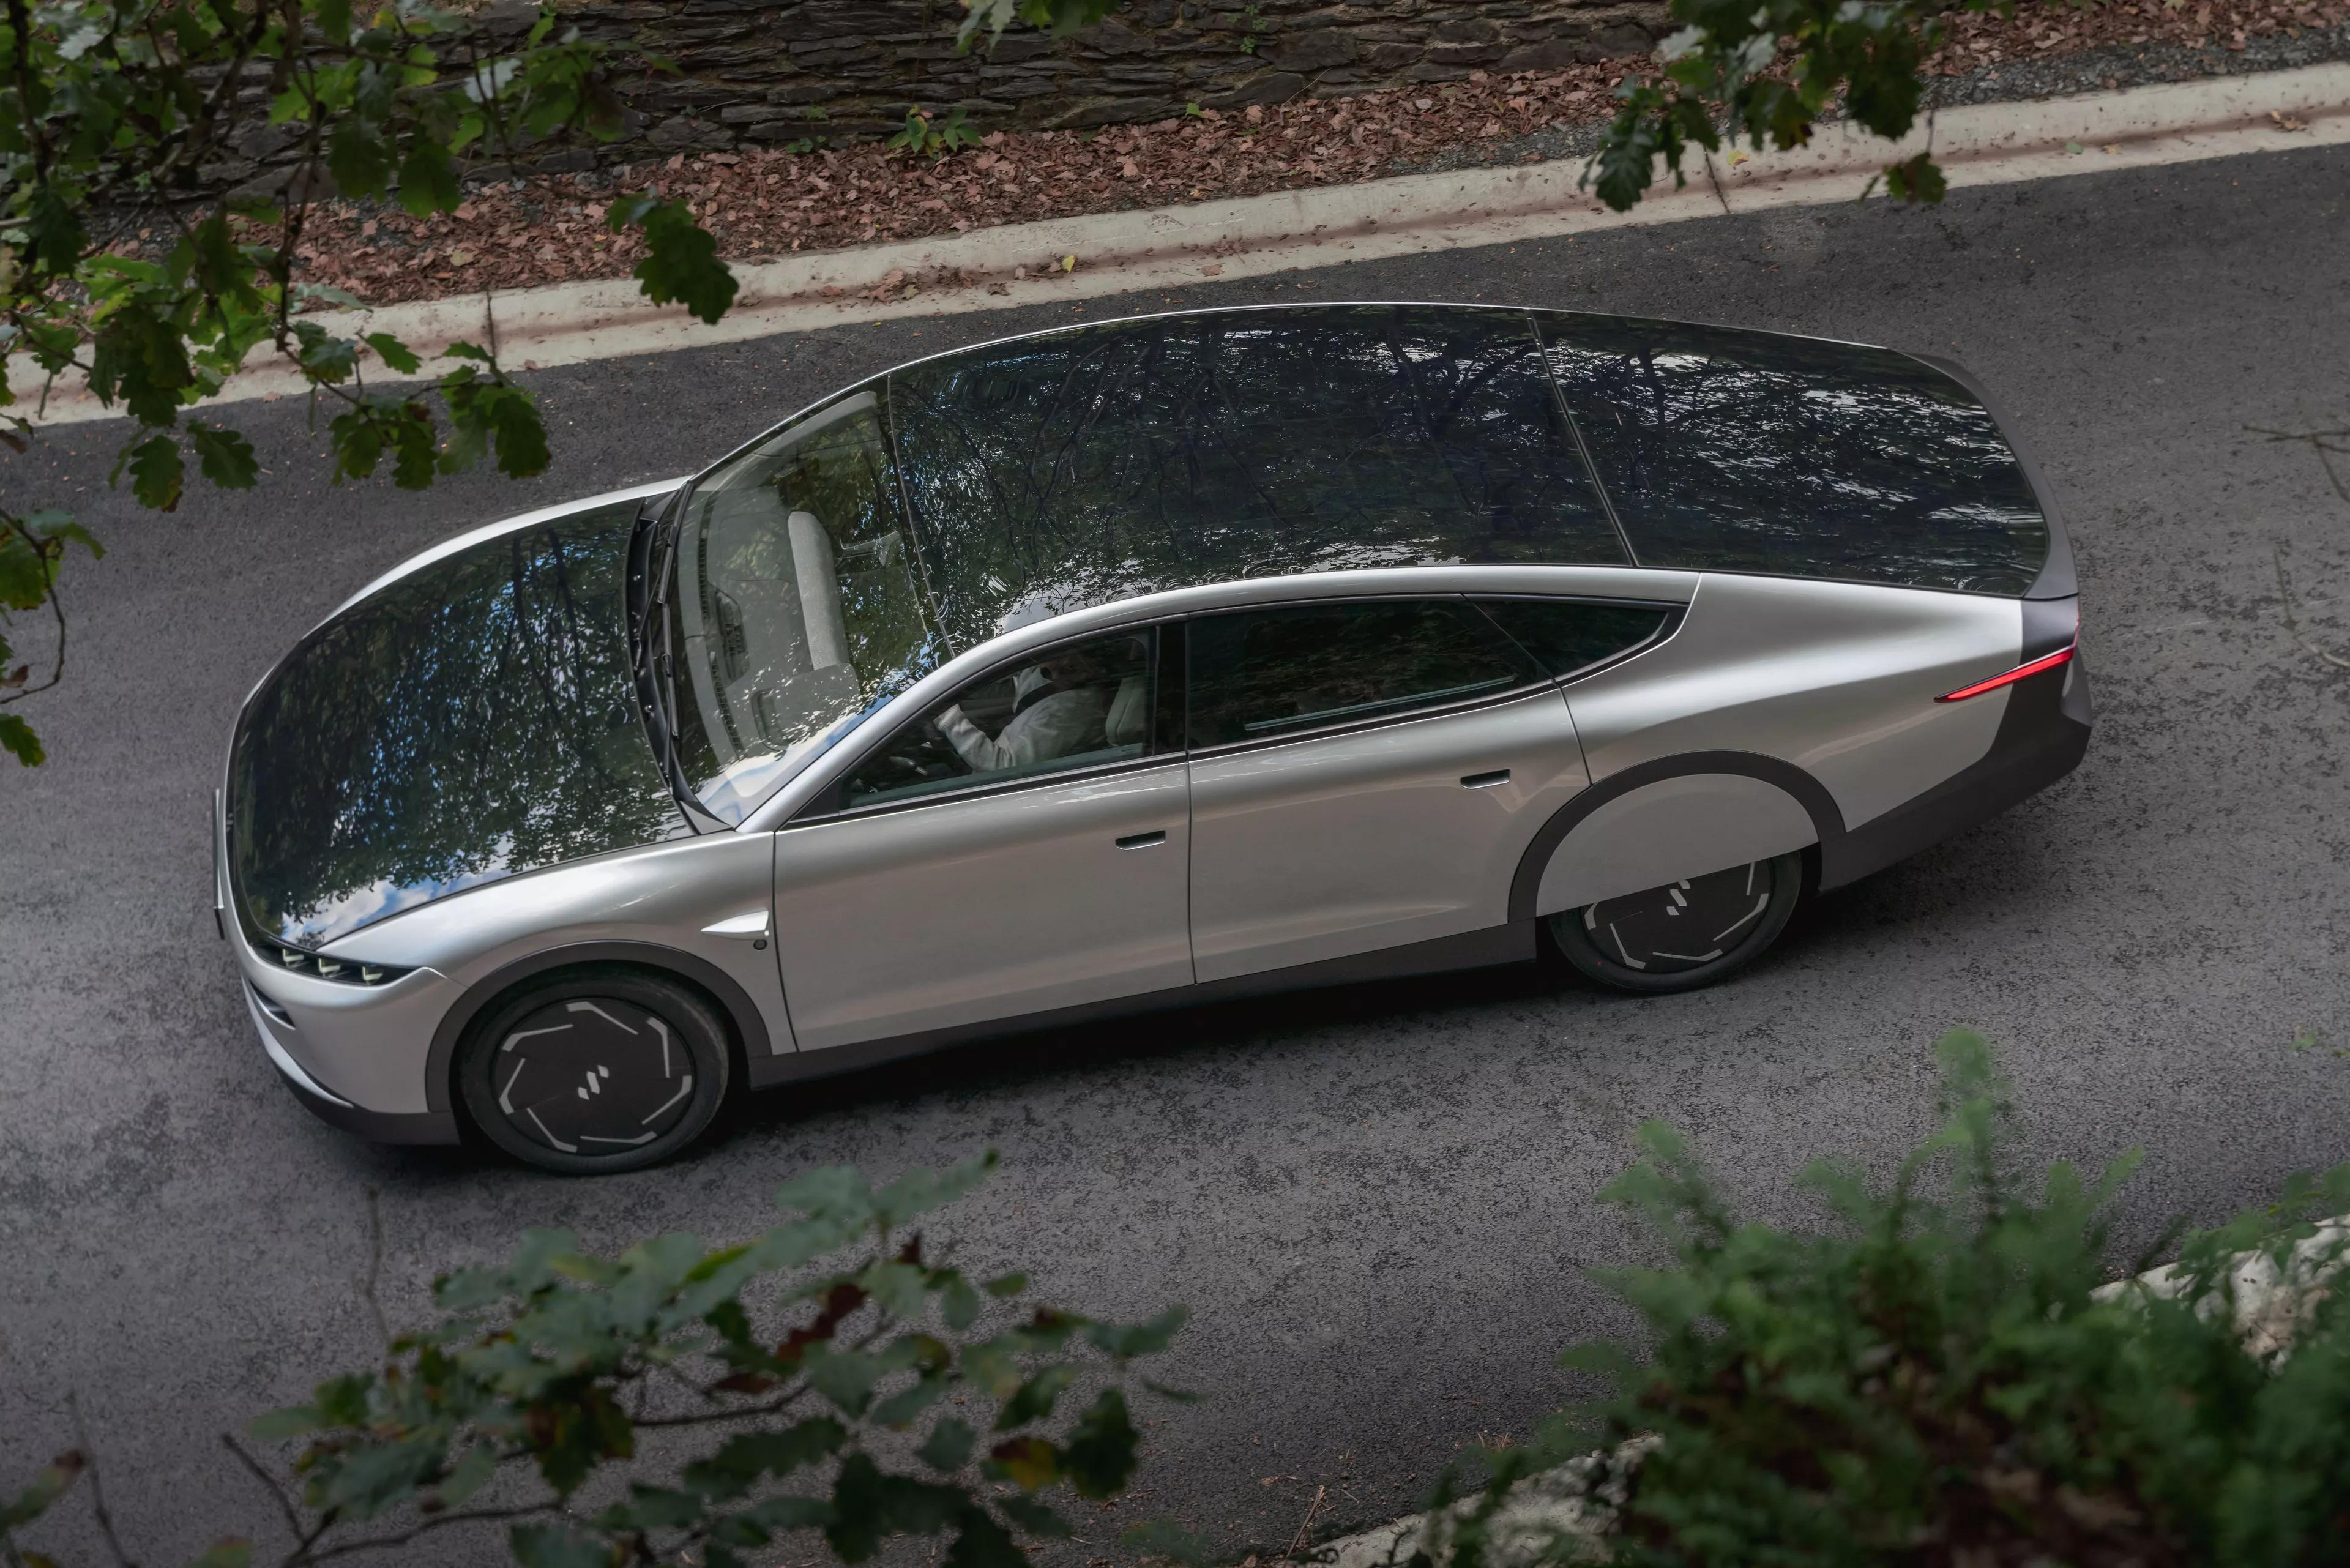
\includegraphics[width=\textwidth]{images/Lightyear_zero.jpg}
    \caption{The Lightyear 0}
    \label{fig:zero}
\end{figure}

In this report we investigate how Lightyear can integrate the \textit{Time Sensitive Networking} technology in the electrical/electronic architecture of their vehicles, the challenges associated with developing such an architecture, we sketch a possible solution to those challenges, and finally we evaluate the feasibility of the proposed solution in the context of a graduation project. The report is structured as follows: Section~\ref{sec:domain} gives some background information on current and future architectures in the automotive domain, explains why Ethernet is sometimes unsuitable for use in an automotive setting and summarizes the main standards of the \textit{Time Sensitive Networking} technology. Section~\ref{sec:problemstatement} describes the problem Lightyear is faced with when implementing \textit{Time Sensitive Networking} into their electrical/electronic architecture. In Section~\ref{sec:sota} an overview is given of the research related to the problem at hand. Section~\ref{sec:researchdescription} explains the question Lightyear is faced with for the transition to a new network architecture and proposes a graduation project contributing an answer to the problem. A development approach is presented, and related risks are identified. Section~\ref{sec:feasibility} describes the experiments and research that were performed to gauge the feasibility of the proposed contribution. Finally, Section~\ref{sec:planning} concludes the preparation project and presents a planning of the graduation project.